\newcommand{\yandex}{\mbox{<<Яндекс>>}}
\newcommand{\yandexbel}{\mbox{<<ЯндексБел>>}}
\newcommand{\rubinplaza}{\mbox{Рубин Плаза}}

\section[Обеспечение пожарной безопасности на предприятии]{Обеспечение пожарной безопасности на предприятии \yandexbel{}}

Целью дипломного проектирования явилась разработка программного средства для обнаружения радиосигналов с помощью SDR-приемника. С его помощью можно сканировать радиоэфир, выделяя наиболее сильные источники сигнала, а также исследовать отдельные частоты, определяя нешумовые последовательности. Аппаратная часть проекта обеспечена приемником на базе software defined radio, что позволяет значительно сократить материальные расходы в сравнении с традиционными системами. В настоящем разделе рассмотрим вопросы, связанные с обеспечением пожарной безопасности в компании \yandexbel{}.

Разработка выполнялась при прохождении преддипломной практики в компании \yandexbel{}. \yandexbel{} --- дочерняя компания \yandex{}. Основным направлением ее деятельности является разработка программного обеспечения. Белорусскому офису всего несколько лет, но сейчас там работает более ста человек и ожидается дальнейший рост. Офис располагается в двух блоках бизнес-центра \rubinplaza{}.

\rubinplaza~--- современный бизнес-центр категории Б. Помимо \yandexbel{} в нем работают команды EPAM Systems, Onliner, БПС-Сбербанк. Планировка здания обеспечивает высокий уровень пожарной безопасности. Каждый офисный блок имеет два выхода. Парадный выход оборудован лифтами и лестницей, пожарный --- только лестницей. На каждом этаже имеется свободный доступ к им обоим. Огнезащитное покрытие конструкций изолирует секции этажа, предотвращая распространение пламени.

Въезд на территорию бизнес-центра контроллируеся охраной. Блокирование проездов и проходов не допускается. Внешняя сторона здания остеклена, что позволяет использовать оконные проемы для экстренного доступа в помещения.

За пожарную безопасность в \yandexbel{} отвечает директор компании. После найма сотрудники проходят инструктаж по установленному противопожарному режиму и мерам безопасности при работе с электрооборудованием. Курение внутри здания запрещено, в каждом помещении установлены пожарные извещатели. Рабочие места организованы таким образом, чтобы организовать беспрепятственный доступ к сетевым фильтрам и проложить кабели электроприборов вне рабочей области людей.

Для отопления помещений используются приборы центрального водяного отопления. Воздухонагревательные элементы объединены в вентиляционную систему здания. Воздуховоды вмонтированы в межэтажные перекрытия и недоступны извне. Электросеть здания также проложена в межсекционных перегородках и межэтажных перекрытиях. Работники компании подключаются к ней через сетевые фильры, защищающие от резких скачков напряжения. В помещениях имеется достаточное количество розеток для подключения всего необходимого электрооборудования.

\begin{figure}
  \begin{center}
    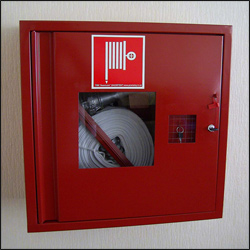
\includegraphics[height=0.4\textheight]{fireplug}
    \caption{Пожарный кран}
    \label{fig:fireplug}
  \end{center}
\end{figure}

В коридорах установлены пожарные краны (\autoref{fig:fireplug}). Ключи к ним находятся в специальных застекленных отсеках и в случае экстренной ситуации могут быть быстро извлечены без посторонней помощи. Двери кабинетов расположены по обе стороны коридора недалеко друг от друга. При таком расположении один пожарный кран может использоваться в нескольких кабинетах, что повышает их удельную эффективность. Более того, они сгруппированы в блоки по 2-4 штуки для тушения сильных возгораний или использования одновременно в нескольких помещениях.

\begin{figure}
  \begin{center}
    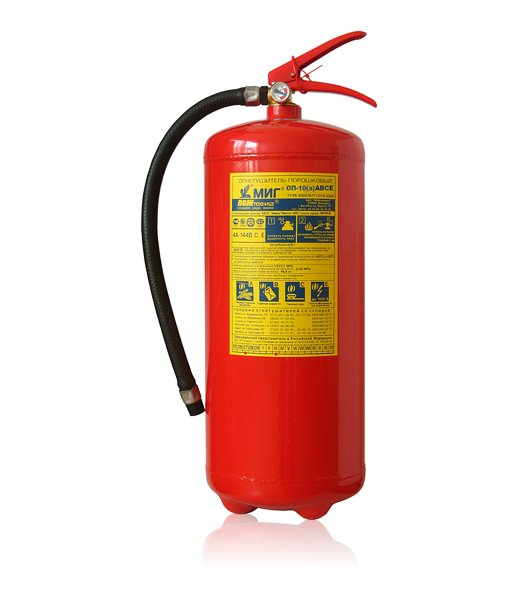
\includegraphics[height=0.4\textheight]{extinguisher}
    \caption{Порошковый огнетушитель \mbox{ОП-10} (з) МИГ М}
    \label{fig:extinguisher}
  \end{center}
\end{figure}

Для оперативного тушения пламени в кабинетах установлены порошковые огнетушители (\autoref{fig:extinguisher}). Они являются самыми распространенными по причине своей универсальности и экономичности: их можно перезарящать и они применяются ко всем источникам воспламенения, для поддержания которых нужен воздух. Огнетушащий порошок не вызывает короткого замыкания электроцепей, что позволяет использовать его в помещении с электрооборудованием под напряжением. Однако, для компьютерной техники это не самый эффективный способ борьбы с огнем, так как происходит значительное загрязнение оборудования порошком и ему требуется чистка. Углекислотные огнетушители лучше справляются с этой задачей --- газ испаряется в окружающую среду без повреждения техники.

В IT компании проблемы с электрооборудованием являются наиболее вероятной угрозой пожарной безопасности. Это персональные компьютеры работников, их личные электроприборы, принтеры и сканеры, серверное помещение --- концентрация электроники очень высока. В условиях такой нагрузки подключаться к электросети нужно через сетевые фильтры. Они оснащены элементом, предохраняющим от скачков напряжения и могут иметь плавкий предохранитель, который размыкает цепь в случае короткого замыкания. Также важно расположение проводов в помещениях --- они проложены вдоль стен и под столами, то есть вне рабочей области людей, если же они протянуты в проходах, пережаты, или изломаны, значительно возрастает вероятность короткого замыкания и поражения людей током. Короткое замыкание вызывает нагрев изоляции проводов, что может привести к ее тлению и распространению огня.

\begin{figure}
  \begin{center}
    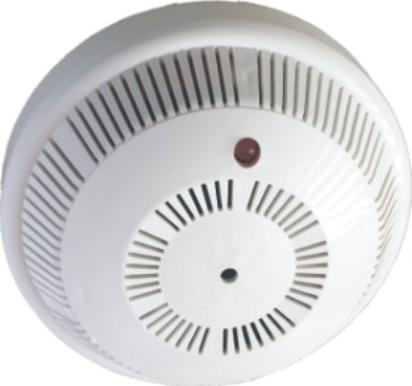
\includegraphics[height=0.4\textheight]{auto_fire_detector}
    \caption{Автономный пожарный извещатель}
    \label{fig:auto_fire_detector}
  \end{center}
\end{figure}

\begin{figure}
  \begin{center}
    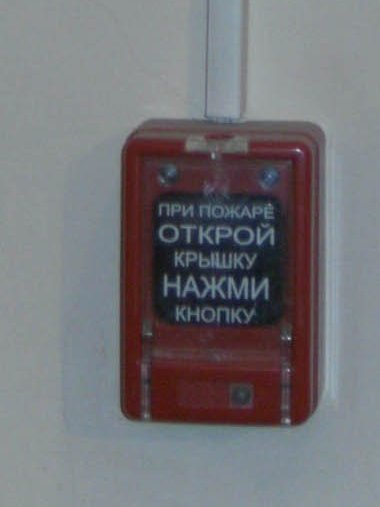
\includegraphics[height=0.4\textheight]{manual_fire_detector}
    \caption{Ручной пожарный извещатель}
    \label{fig:manual_fire_detector}
  \end{center}
\end{figure}

Каждый кабинет оборудован пожарными дымовыми оптико-электронными точечными извещателями \mbox{ИП212-02М1} (\autoref{fig:auto_fire_detector}). Дымовые извещатели работают по принципу контроля оптических свойств окружающей среды. Они обнаруживают возгорание по изменению светового потока, то есть прозрачности воздуха или по яркости отраженного света от частиц дыма. Оптико-электронные датчики легко фиксируют дым серого цвета, образующийся на начальной стадии тления. В коридорах дополнительно установлены ручные пожарные извещатели \mbox{ИП 5-2Р} (\autoref{fig:manual_fire_detector}). С их помощью человек, обнаруживший признаки возгорания, может подать сигнал о пожаре не дожидаясь срабатывания автоматических средств.

\begin{figure}[h]
  \begin{center}
    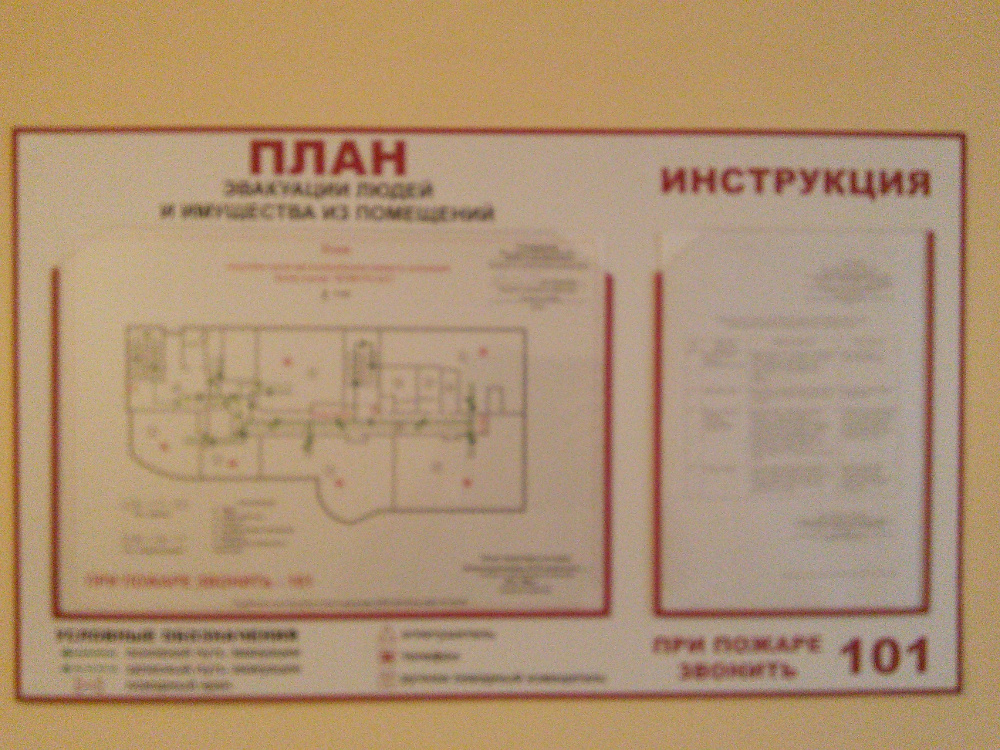
\includegraphics[height=0.4\textheight]{evacuation_plan}
    \caption{План эвакуации}
    \label{fig:evacuation_plan}
  \end{center}
\end{figure}

Если с огнем не удается справится своими силами, необходимо вывести людей из здания. На каждом этаже висят план эвакуации и инструкция (\autoref{fig:evacuation_plan}). Они содержит информацию, необходимую в экстренной ситуации --- номер телефона пожарной службы, краткое руководство по действиям в случае ЧП, расположение огнетушителей и пожарных кранов и порядок эвакуаций людей и материальных ценностей.

Таким образом, изложенные выше предложения обеспечивают пожарную безопасность в компании \yandexbel{}.
